\documentclass[12pt,a4paper]{article}

% To use this template make changes to following:
% 1. Fill-ables section.
% 2. Instructions.
% 3. Marks table.
% 4. Actual questions.

% ================================ 1. Fill-ables ================================
\newcommand\University{National University of Computer and Emerging Sciences}
\newcommand\Department{School of Engineering}
\newcommand\Campus{Islamabad Campus}
\newcommand\Semester{Summer 2014}
\newcommand\Exam{Sessional Exam}
\newcommand\Subject{EE308--Microwave Engineering}
\newcommand\ExamDate{Saturday, July 12, 2014}
\newcommand\InstructorOne{Attique Dawood}
\newcommand\InstructorTwo{}
\newcommand\InstructorThree{\null}
\newcommand\TotalTime{02 Hours}
\newcommand\TotalMarks{100}
\newcommand\TotalQuestions{5}
\newcommand\TotalPages{\pageref{LastPage}} % Automatic: No need to change this.
% Marks of each question
\def\Qone{20}
\def\Qtwo{20}
\def\Qthree{20}
\def\Qfour{20}
\def\Qfive{20}
\def\Qsix{0}
\def\Qseven{0}
\def\Qeight{0}
\def\Qnine{0}
\def\Qten{0}
% ============================================================================

% ============== 2. Packages ==============
\usepackage{amsmath}
\usepackage{float}
\usepackage{graphicx}
\usepackage[hyphens]{url}
\usepackage[hidelinks]{hyperref}	% Clickable links to figures, references and urls.
\usepackage{lastpage}
\usepackage{array}
\usepackage{fancyhdr}
\usepackage{afterpage}
% Drawing packages.
\usepackage{pgf}
\usepackage{tikz}
% Listings for formatting code.
\usepackage{listings}
\usepackage{textcomp}

% General listings options.
\lstset{breaklines=true, basicstyle=\footnotesize\ttfamily, tabsize=4, numbers=left, stepnumber=1, frame=none, showstringspaces=false, upquote=true}
% C++ specific high-lighting. Comments are 50/50 shades of green/black and strings coloured with 60/40 red/black mixture.
\lstset{language=[ISO]C++, commentstyle=\color{green!50!black}, keywordstyle=\color{blue}, stringstyle=\color{red!60!black}}

% Table cell alignment directives.
\newcolumntype{L}[1]{>{\raggedright\let\newline\\\arraybackslash\hspace{0pt}}m{#1}}
\newcolumntype{C}[1]{>{\centering\let\newline\\\arraybackslash\hspace{0pt}}m{#1}}
\newcolumntype{R}[1]{>{\raggedleft\let\newline\\\arraybackslash\hspace{0pt}}m{#1}}

% Line spacing.
\def\SingleSpacing{\def\baselinestretch{1}\large\normalsize}
\def\DoubleSpacing{\def\baselinestretch{1.5}\large\normalsize}

% Margins.
\setlength{\oddsidemargin}{0in}
\setlength{\evensidemargin}{0in}
\setlength{\headheight}{28pt}
\setlength{\headsep}{2.5pt}
\setlength{\topmargin}{-60pt}
\setlength{\textwidth}{6.5in}
\setlength{\textheight}{10.75in} % Actual: 10.75in

% ============================= 3. Header and Footer ============================
\pagestyle{empty}
% Header
\chead
{
	{\large\textbf{\University}}\\
	\begin{minipage}{0.45\textwidth}
	\begin{center}
	{\small\textbf{\Department}}
	\end{center}
	\end{minipage}
	\begin{minipage}{0.45\textwidth}
	\begin{center}
	{\small\textbf{\Campus}}
	\end{center}
	\end{minipage}
}
% Footer
\lfoot{{\small\Exam}}
\cfoot{{\small\Semester}}
\rfoot{{\small Page \textbf{\thepage}~of \textbf{\TotalPages}}}
\renewcommand{\headrulewidth}{0.4pt}
\renewcommand{\footrulewidth}{0.4pt}
% ================================= 4. Front Page ===============================
\begin{document}
% A cute macro to add up marks of all individual questions. Uncomment if you want to use this.
\pgfmathtruncatemacro\TotalMarks{\Qone+\Qtwo+\Qthree+\Qfour+\Qfive+\Qsix+\Qseven+\Qeight+\Qnine+\Qten}
% Use this macro if marks are in decimal points
%\newcommand\TotalMarks{\pgfmathsetmacro\TotalMarks{\Qone+\Qtwo+\Qthree+\Qfour+\Qfive+\Qsix+\Qseven+\Qeight+\Qnine+\Qten}}
\begin{minipage}[t]{0.6\textwidth}
\begin{flushleft}
\DoubleSpacing
{\Large\textbf{\Subject}}\\
{\normalsize\ExamDate}\\
{\large\textbf{Course Instructor}}\\
{\normalsize\InstructorOne}\\
{\normalsize\InstructorTwo}
{\normalsize\InstructorThree}
\end{flushleft}
\end{minipage}
\begin{minipage}[t]{0.01\textwidth}
~
\end{minipage}
\begin{minipage}[t]{0.325\textwidth}
\DoubleSpacing
{\normalsize Serial No:}\\
{\Large\textbf{\Exam}}\\
{\large\textbf{Total Time: \TotalTime}}\\
{\large\textbf{Total Marks: \TotalMarks}}\\[1cm]
\rule{5cm}{0.2mm}\\[-0.25cm]
{\small Signature of Invigilator}
\end{minipage}
\SingleSpacing
~\\[1.5cm] % Extra space.
\rule{7cm}{0.2mm}~\rule{2.5cm}{0.2mm}~\rule{2cm}{0.2mm}~\rule{4.5cm}{0.2mm}\\
{\small Student Name\hspace{4.75cm}Roll No\hspace{1.35cm}Section\hspace{0.95cm}Signature}\\[1cm]
% ============================ 5. Instructions ==================================
\textbf{DO NOT OPEN THE QUESTION BOOK OR START UNTIL INSTRUCTED.}\\
\textbf{Instructions:}
\begin{enumerate}
\itemsep0em
\item Verify at the start of the exam that you have a total of \TotalQuestions~questions printed on \TotalPages~pages including this title page.
\item Attempt all questions on the question-book and in the given order.
\item The exam is closed books, closed notes. Please see that the area in your threshold is free of any material classified as `useful in the paper' or else there may be a charge of cheating.
\item Read the questions carefully for clarity of context and understanding of meaning and make assumptions wherever required, for neither the invigilator will address your queries, nor the teacher/examiner will come to the examination hall for any assistance.
\item Fit in all your answers in the provided space. You may use extra space on the last page if required. If you do so, clearly mark question/part number on that page to avoid confusion. 
\item Use only your own stationery and calculator. If you do not have your own calculator, use manual calculations. 
\item Use only permanent ink-pens. Only the questions attempted with permanent ink-pens will be considered. Any part of paper done in lead pencil cannot be claimed for checking/rechecking.
\end{enumerate}
% =============================== 6. Marks Table ================================
\begin{table}[H]
\begin{center}
\vspace{0.3cm}
	{\footnotesize \begin{tabular}{|C{1.8cm}|C{0.75cm}|C{0.75cm}|C{0.75cm}|C{0.75cm}|C{0.75cm}|c|}
	\hline
		\rule{0pt}{4.6ex} & Q-1 & Q-2 & Q-3 & Q-4 & Q-5 & \textbf{Total}\\[-0.5ex]
		\hline
		\rule{0pt}{2.5ex}\textbf{Total Marks}& \Qone & \Qtwo & \Qthree & \Qfour & \Qfive & \TotalMarks\\
		\hline
		\rule{0pt}{2.5ex}\textbf{Marks Obtained}& & & & & &\\
	\hline
	\end{tabular}}
\end{center}
\end{table}
{\small \textbf{Vetted By: \rule{6cm}{0.2mm} Vetter Signature: \rule{4.5cm}{0.2mm}}}
\setlength{\textheight}{10.5in}
\newpage
\pagestyle{fancy}
% ================================== 7. Questions ===============================
\noindent\textbf{Question 1: \hfill $2\times10=$\Qone~marks}\\
a. What is the significance of Microwave Engineering with respect to Circuit Theory? Under what conditions Circuit Theory cannot be used for circuit analysis and Microwave techniques are necessary?\\[12.5cm]
b. A quarter--wave transformer is used to match a transmission line with $Z_0=60 \Omega$ with a load $Z_L=120 \Omega$. Find the characteristic impedance of quarter--wave transformer line that will result in a match.
\newpage
\noindent \textbf{Question 2: \hfill \Qtwo~marks}\\
A plane wave travelling in free space along $+z$ direction is normally incident on a medium with $\epsilon=9\epsilon_0$ and $\mu=\mu_0$. The incident electric field is given by $\mathrm{\textbf{E}}=2\cos(\omega t-\beta z)\hat y$ V/m. Find the reflected and transmitted electric fields. Also find incident, reflected and transmitted magnetic fields.
\newpage
\noindent\textbf{Question 3: \hfill \Qthree~marks}\\
A $120+j80\Omega$ load is connected to a $50\Omega$ transmission line. Use manual calculations to find,
\begin{itemize}
\item[a.] $\Gamma$
\item[b.] VSWR
\item[c.] $Z_{in}$ at $0.3\lambda$ from load
\item[d.] $Z_{in}$ at generator if line is $0.6\lambda$ long.
\end{itemize}
\newpage
\noindent\textbf{Question 4: \hfill \Qfour~marks}\\
Repeat Question 3 using Smith Chart. Also, find values of $V_{max}$ and $V_{min}$ in addition to their locations on the line.
\newpage
\begin{figure}[H]
\centering
\vspace{4cm}
\hspace*{-1.6cm}
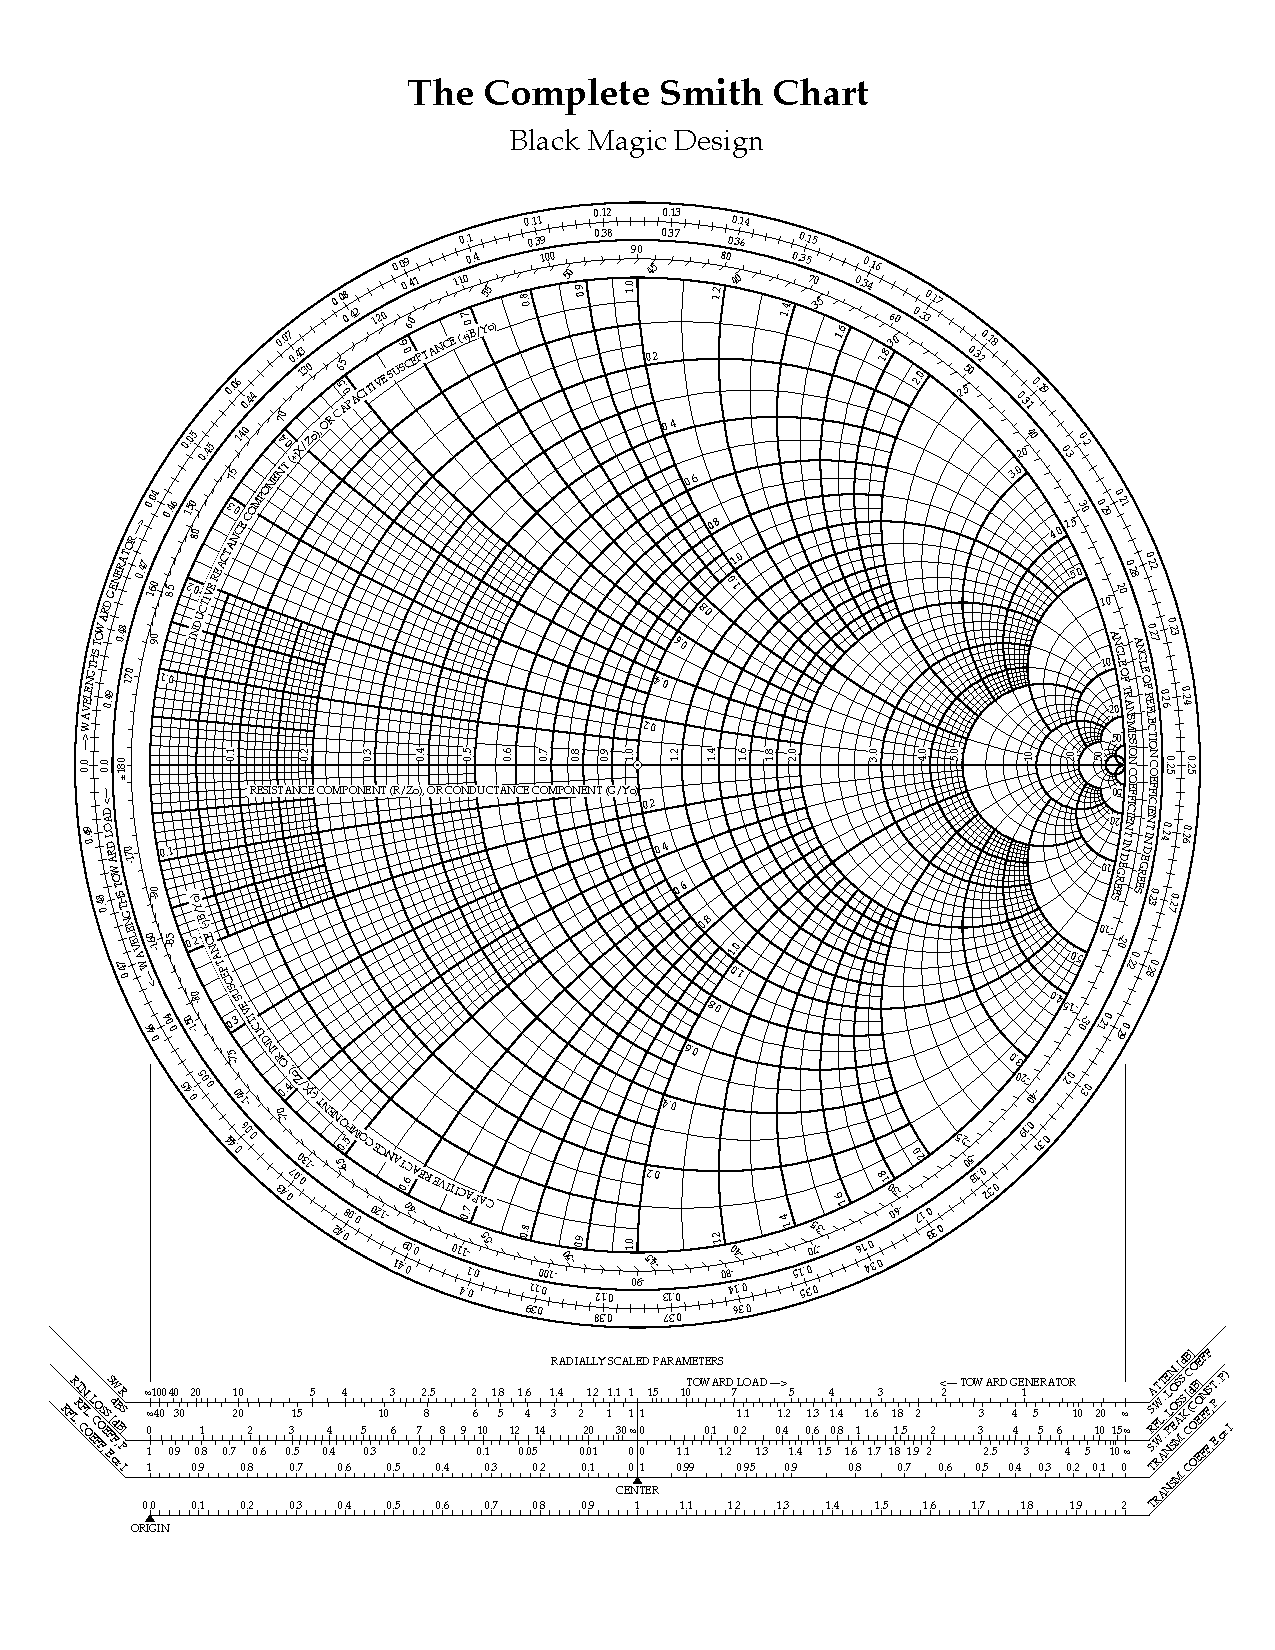
\includegraphics[scale=1.0,trim=1cm 2cm 1cm 3cm, clip]{./SmithChart}
\label{fig:SmithChart1}
\end{figure}
\newpage
\noindent\textbf{Question 5: \hfill \Qfive~marks}\\
An antenna with $Z_L=80-j40\Omega$ is to be matched to a $100\Omega$ lossless transmission line using shorted stub. Find the distance from antenna, $l$, at which stub is to be attached and the length of stub $d$. Of two possible solutions only one is required.
\newpage
\begin{figure}[H]
\centering
\vspace{4cm}
\hspace*{-1.6cm}
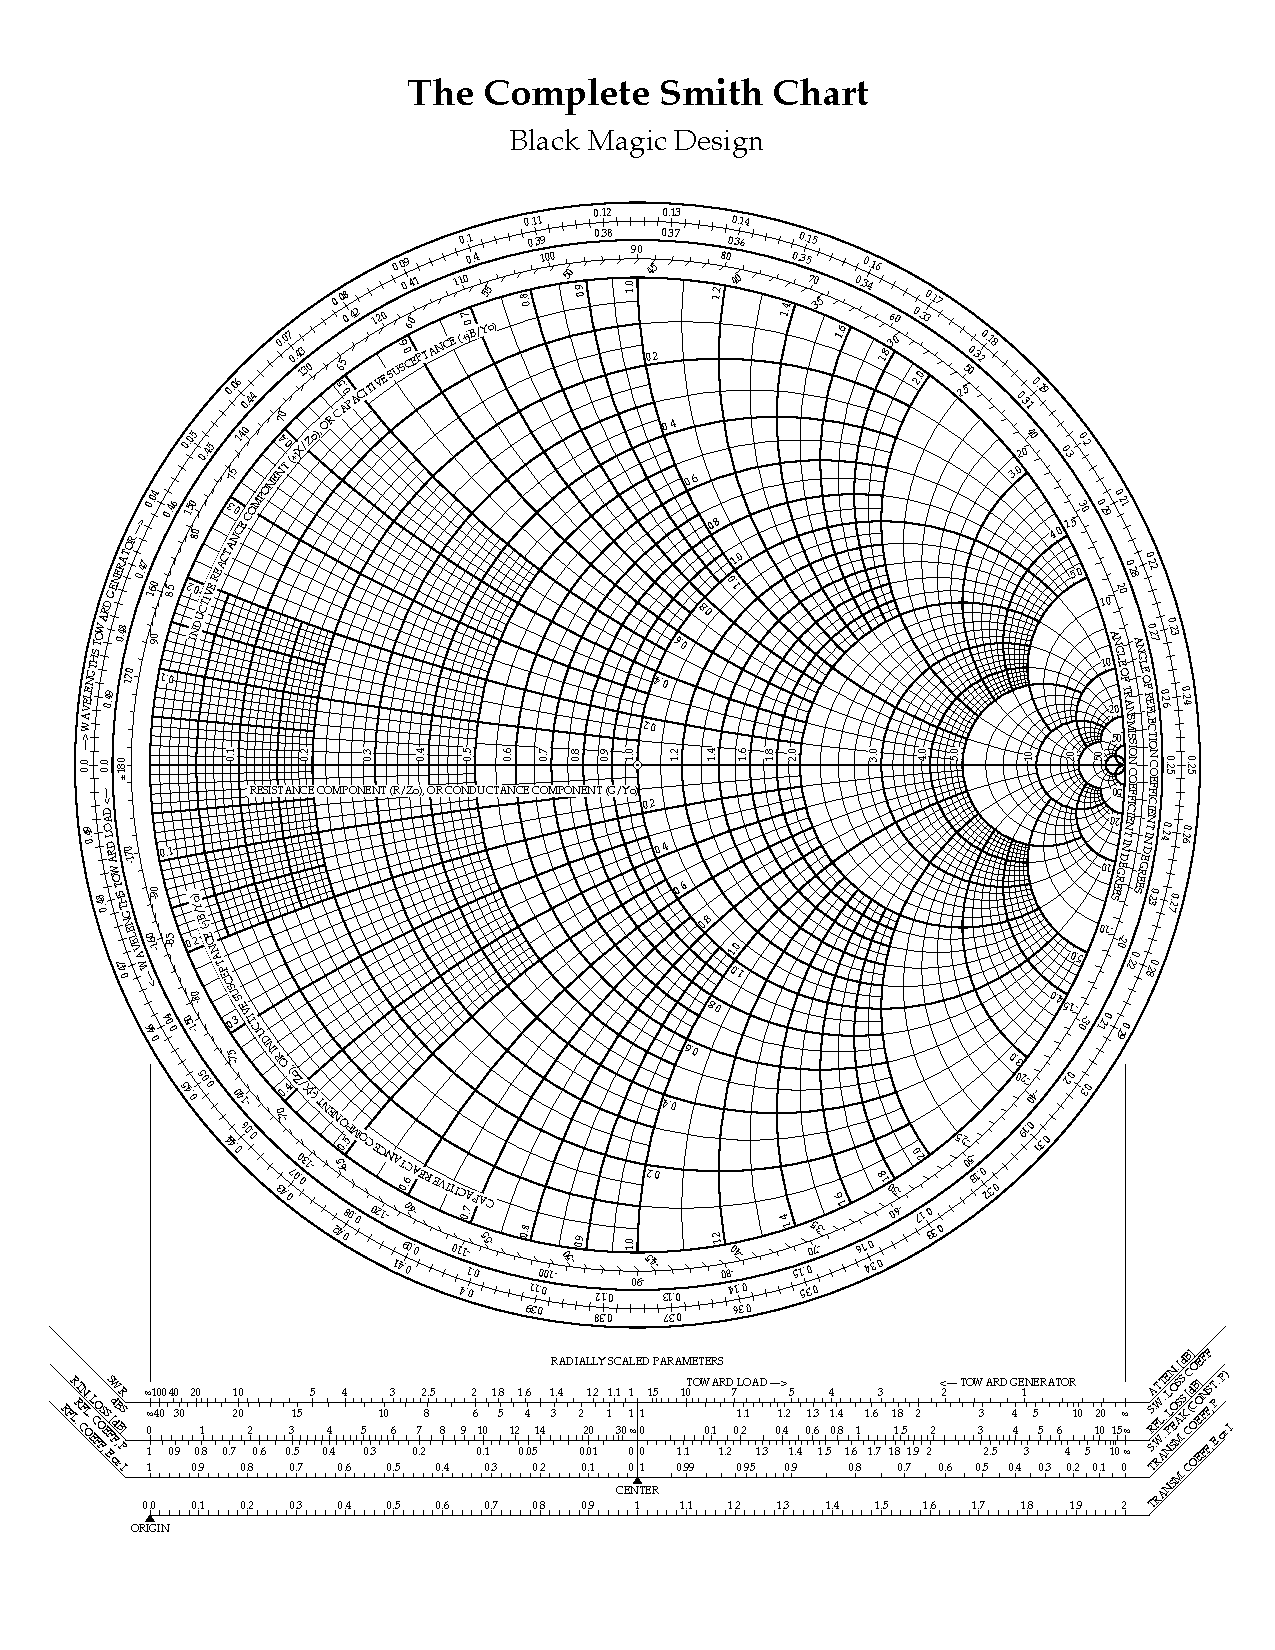
\includegraphics[scale=1.0,trim=1cm 2cm 1cm 3cm, clip]{./SmithChart}
\label{fig:SmithChart2}
\end{figure}
\newpage
\begin{figure}[H]
\centering
\vspace{4cm}
\hspace*{-1.6cm}
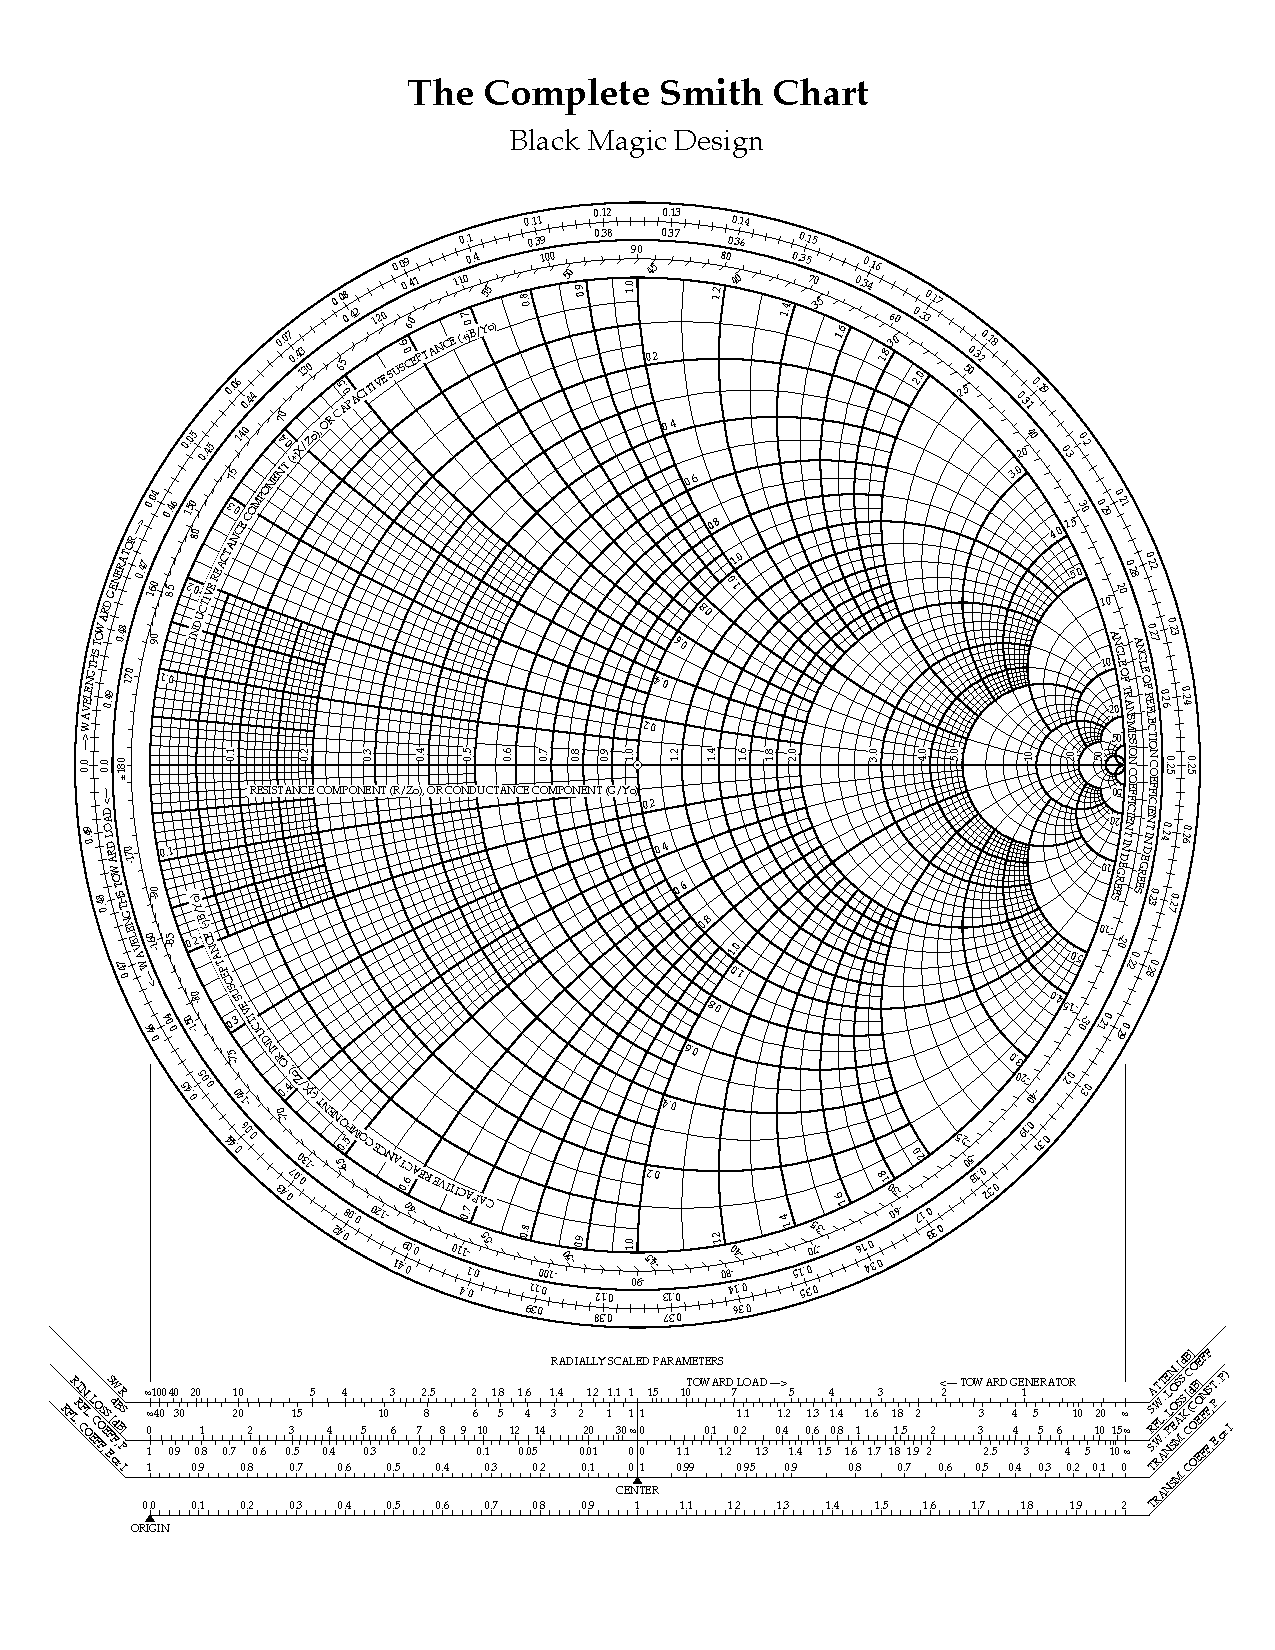
\includegraphics[scale=1.0,trim=1cm 2cm 1cm 3cm, clip]{./SmithChart}
\label{fig:SmithChart3}
\end{figure}
\end{document}